\chapter{Applications to Neuromorphic Hardware}
\label{chapt:results}

Nengo and the NEF provide a useful toolkit for programming recurrently coupled networks of spiking neurons to carry out the computations of algorithms formulated as dynamical systems.
The CPU backend is immensely useful for rapidly prototyping ideas, testing hypotheses, and experimenting with small-scale models on the order of a few thousand neurons.
However, for much larger models such as Spaun~\citep{eliasmith2012}, its 2.5~million neurons require about 2.5~hours of compute time per $1$~second of simulation time, that is $\approx \numprint{9000}$ times slower than real-time~\citep{stewart2014large, mundy2016real}.
As a result, one must turn to specialized hardware such as GPUs, FPGAs, or neuromorphic architectures, in order to carry out much larger simulations of spiking neural networks (section~\ref{sec:neuromorphic}).

For example, in our work in collaboration with \citet{knight2016}, we demonstrate that a heteroassociative memory network deployed on SpiNNaker takes a \emph{constant} amount of time per association, while the exact same network takes a linear amount of time per association on a CPU.\footnote{%
The number of neurons were scaled linearly in the number of associations.}
At its largest instantiation of \numprint{100000} neurons, the SpiNNaker simulation is more than $150$ times faster than a CPU, due to the massive parallelism afforded by the architecture.
This demonstration is encouraging to see, as it illustrates the potential for these methods to scale up and take full advantage of the distributed nature of spiking computation, while leveraging the power of dynamical systems to learn synaptic weights with both unsupervised (section~\ref{sec:unsupervised}) and supervised (section~\ref{sec:supervised}) learning rules.

However, there are very few examples of \emph{functional} large-scale models running on neuromorphic hardware.
We believe that this surprising lack of scale---in a field that was essentially created to solve a problem in scaling---is primarily due to a lack of co-designed NEF-like frameworks for translating computations, specified in some high-level language (e.g.,~coupled differential equations), onto distributed networks of physically coupled devices.
These frameworks must be correct, scalable, complete, robust, extensible, and finally realized on the physical hardware itself, in order to be ultimately useful (section~\ref{sec:nef-suitability}).
In the case of the NEF, this criteria has been validated by many of the extensions and analyses throughout this thesis, as well as by past work compiling networks onto
Neurogrid~\citep{dethier2011brain},
SpiNNaker~\citep{mundy2015, mundy2016real, knight2016},
TrueNorth~\citep{fischl2018},
and many other architectures~\citep{naylor2013managing, bekolay2014, corradi2014, wang2014compact, berzish2016, wang2017neuromorphic, rasmussen2018nengodl, blouw2018a}.
% support the translation of computations specified in some high-level language (e.g.,~coupled differential equations), onto distributed networks of physically coupled devices.

However, at time of writing, the Nengo \emph{backends} for Braindrop~\citep{braindrop2019} and Loihi~\citep{nengoloihi} are brand new---as are the chips themselves~\citep{neckar2018braindrop, davies2018loihi}---and thus currently fall short of their promise to realize \emph{large-scale} functional SNNs in neuromorphic hardware.
For the case of Braindrop, its shortcoming is mainly by design: the chip is $0.65$\,mm${}^2$ and implements $\numprint{4096}$ neurons.
It is a proof-of-concept prototype for research, that can in principle be tiled to scale to much larger models in the future and tailored towards the requirements of some application space.
For the case of Loihi, due to a combination of a lack of hardware support for factorized weight matrices, and limitations on connectivity and memory, the maximum recurrently connected pool size is $342$ neurons.\footnote{%
Determined empirically using the \texttt{nengo-loihi==0.5.0} emulator.}
And with current software workarounds, the feed-forward precision stops scaling in Nengo-Loihi after about $400$ neurons.
Nevertheless, this is the first and only software abstraction to currently make use of Loihi~\citep{blouw2018a} outside of Intel~\citep{lin2018mapping}, and it is under active development.
We expect this to get significantly better with time.

%The end-to-end design and fabrication of custom hardware is an extremely costly and complex process that demands a variety of skill-sets from a large number of people.
Nevertheless, these two architectures---Braindrop and Loihi---represent significant milestones in the evolution of neuromorphic hardware.
The first, Braindrop, consumes energy roughly equivalent to $381$\,fJ per synaptic operation, for typical network configurations, or about $10$--$20$ times more than the human brain (see section~\ref{sec:neuromorphic}).
The second, Loihi, consumes about $24$\,pJ per synaptic operation, or about $50$--$100$ times more than Braindrop, but offers determinism and an unparalleled degree of flexibility given its power budget.
At the same time, these two neuromorphic hardware architectures are about as different from one another as two could be in the space of neuromorphic computing, with each posing very different sets of challenges when it comes to compiling NEF networks.

The goal of this chapter is to demonstrate that the fundamentals for systematically programming neuromorphic hardware are in place.
With the theoretical guarantees provided by chapter~\ref{chapt:analysis}, the methods for programming dynamical systems in chapter~\ref{chapt:methodology}, the extensions of chapter~\ref{chapt:nef-extensions}, and the functional capabilities of dynamical systems such as those explored in chapter~\ref{chapt:delays} -- we are confident that in principle these methods can scale to Spaun's 6.6~million neurons~\citep{choo2018} and beyond.
%However, since we only currently have room for a few hundred neurons, there is only so much that we can do.
%For example, \citet{blouw2018a} has shown impressive power reduction for a keyword spotter written using Nengo~DL~\citep{rasmussen2018} on Loihi.
Thus, we focus on demonstrating the principles of the NEF, and a few of its extensions, applied to two fundamental---but admittedly small-scale---dynamical systems.
These dynamical systems are described in the same high-level language of Nengo, but mapped onto two vastly different state-of-the-art neuromorphic architectures: Braindrop and Loihi.

\section{Integrator}
\label{sec:integrator}

The integrator, $\theta \dot{\V{x}}(t) = \V{u}(t)$, is a dynamical system used extensively by Spaun~\citep{eliasmith2012} and many other NEF and SPA models~\citep[][to name a few]{singh2004, trujillo2014a, rasmussen2017} for cognitive tasks involving working memory (also see section~\ref{sec:dynamics-language} for a brief review).
This system persists information about the history of an input signal, starting from $t_0$ and extended indefinitely throughout time, as characterized by the solution to its differential equation,
$$\V{x}(t) = \V{x}(t_0) + \frac{1}{\theta} \int_{t'=t_0}^{t} \V{u}(t')\, dt' \text{.}$$
The parameter $\theta$ is a system-level time-constant that controls how quickly the memory integrates new information.\footnote{%
This parameter is useful for dimensional analysis, when considering the transfer function, $\frac{\V{X}(s)}{\V{U}(s)} = \left( \theta s \right)^{-1}$, and in determining the precision of the system: $n$ scales as $\bigoh{\theta^{-2}}$ (see Table~\ref{tab:scalability}).}
For example, beginning from an initial state of $\V{x}(t_0) = \V{0}$, if we hold the input constant at $\V{u}(t) = \V{v}$ for $\theta$ seconds ($t_0 < t \le t_0 + \theta$), and then clamp the input to $\V{u}(t) = \V{0}$ thereafter ($t > t_0 + \theta$), then $\V{x}(t) = \V{v}$ will ``store'' the vector $\V{v}$ indefinitely.

More generally, any finite set of nonlinear differential equations can be described as the integration of an input vector that is some nonlinear function of the state-vector---augmented to also include $\V{u}(t)$---as in $\theta \dot{\V{x}}(t) = \V{f}\left({\V{x}(t)}\right)$.
The nonlinearity $\V{f}(\cdot)$ may then be supported by a pool of neurons encoding the state-vector, as explained in section~\ref{sec:nef}.
Indeed, this is the essential observation of Principle 3; dynamical systems may be reduced to integration.
Thus, the integrator is a basic component used to implement sophisticated nonlinear dynamical transformations, such as those involved in adaptive motor control~\citep{dewolf2016}.
We therefore use the integrator, implemented by a pool of spiking neurons using the methods of the NEF, as a benchmark for evaluating the ability of neuromorphic hardware to implement generic dynamical systems.

In Figure~\ref{fig:integrator-neuromorphic}, we instantiate a one-dimensional integrator ($\theta = 1$\,s) on both Braindrop (1024 neurons) and Loihi (256 neurons).
%\footnote{%
%We use four times fewer neurons on Loihi versus Braindrop, as increasing the pool size leads to a bug in the \texttt{nengo-loihi}~v0.4.0 software.}
In both cases, the input signal is a white noise test signal, band-limited to $1$\,Hz.
Both the ideal and the spiking activity are filtered with a lowpass ($\tau = 200$\,ms).
We report the mean output's 95\% confidence intervals, bootstrapped from $200$ trials lasting $10$ seconds each.
We run a large number of trials with random configurations of the network on the same input, in order to assess overall robustness, and to reveal any systemic biases in the error or drift.

\begin{figure}
  \centering
  \begin{subfigure}{.5\textwidth}
    \centering
    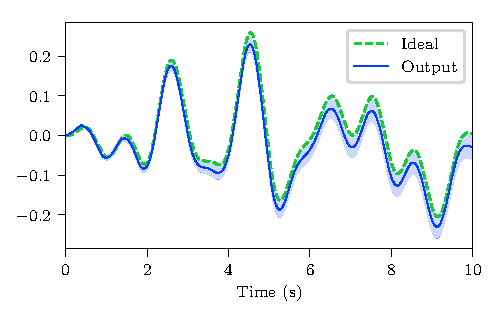
\includegraphics[width=\linewidth]{braindrop-integrator}
    \caption{Braindrop}
    \label{fig:braindrop-integrator}
  \end{subfigure}%
  \begin{subfigure}{.5\textwidth}
    \centering
    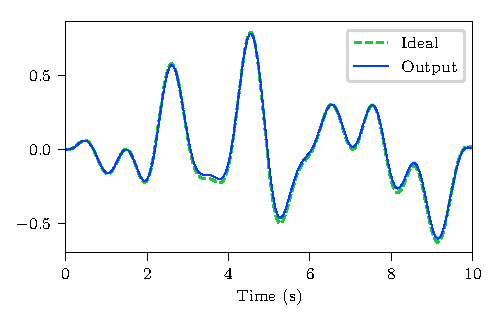
\includegraphics[width=\linewidth]{loihi-integrator}
    \caption{Loihi}
    \label{fig:loihi-integrator}
  \end{subfigure}
  \caption[Dynamical integration on Braindrop and Loihi.]{
    An integrator running on state-of-the-art neuromorphic hardware.
    The ideal solution is plotted against the mean's 95\% confidence interval, bootstrapped from $200$ trial simulations.
    (a)~Nengo Braindrop implementation, reproduced from \citet[][Figure~15]{braindrop2019}, using \numprint{1024} neurons. 
    (b)~Nengo Loihi (v0.5.0) implementation, using \numprint{256} neurons.
    Loihi simulations performed by Xuan Choo from Applied Brain Research, Inc.
    See text for details.
  }\label{fig:integrator-neuromorphic}
\end{figure}

On Braindrop (see Figure~\ref{fig:integrator-neuromorphic}~(a), reproduced from \citet[][Figure~15]{braindrop2019}), we compensate for the distribution of synaptic time-constants, arising from transistor mismatch in the analog circuitry, using the methods of \citet{voelker2017iscas}, detailed in section~\ref{sec:nonlinear-extensions} and~\ref{sec:mismatch}.
We do so by first measuring the time-constants, and then targeting them individually with the specific transform given by our extensions.
The chip is configured to maximize the synaptic time-constants; the empirically measured mean is $179.3$\,ms, with a standard deviation of $53.8$\,ms.
To help account for temperature-induced variability---manifesting as slowly-changing shifts to the effective tuning curves~\citep{abrams2017}---we also retrain the weights every 10 simulations directly from the spike data, collected using a separate training signal.
The rest of the mapping is handled by the Nengo-Braindrop backend~\citep{neckar2018optimizing, braindrop2019}.

On Loihi (see Figure~\ref{fig:integrator-neuromorphic}~(b)), we set $\tau = 200$\,ms, and use the methods of section~\ref{sec:linear-extensions} to discretize the integrator according to the simulation time-step ($\dt{} = 1$\,ms).
We also use non-leaky neurons (integrate-and-fire), as this provides the best accuracy (see section~\ref{sec:poisson-spiking}).
Weight matrices are left unfactored.
Lastly we move the input synapse onto the spike-generator from host to chip, and uniformly initialize the states of the spike-generators to satisfy the uniform ISIP criteria (Theorem~\ref{thm:correctness}).
The rest of the mapping is handled by the Nengo-Loihi backend~\citep{nengoloihi}.

In both cases, the 95\% confidence intervals include the ideal across nearly the entire $10$\,s simulation.
This implies that the sum of any error, whether related to spiking, representation, or otherwise, has a mean value of approximately zero.
We remark that Loihi gives much more consistent trial-to-trial results, due to the all-digital nature of the chip, determinism, and lack of temperature-induced variability.
Advanced methods that can be used to provide temperature-invariant decodes in Braindrop have been recently developed by \citet{reidpint2019}, although they require external measurements of the device's temperature, and thus were not employed in this experiment.

\section{Delay Network}
\label{sec:neuromorphic-dn}

\begin{figure}
  \centering
  \begin{subfigure}{.5\textwidth}
    \centering
    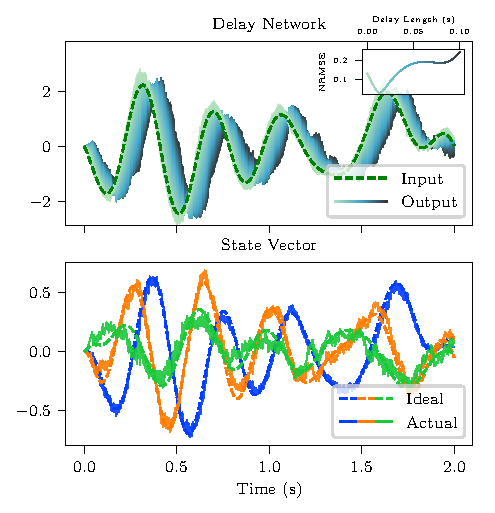
\includegraphics[width=\linewidth]{dn-braindrop}
    \caption{Braindrop}
    \label{fig:dn-braindrop}
  \end{subfigure}%
  \begin{subfigure}{.5\textwidth}
    \centering
    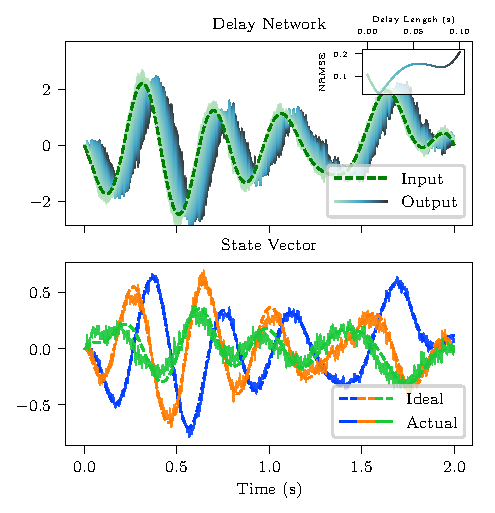
\includegraphics[width=\linewidth]{dn-loihi}
    \caption{Loihi}
    \label{fig:dn-loihi}
  \end{subfigure}
  \begin{subfigure}{\textwidth}
    \centering
    \vspace{2em}
    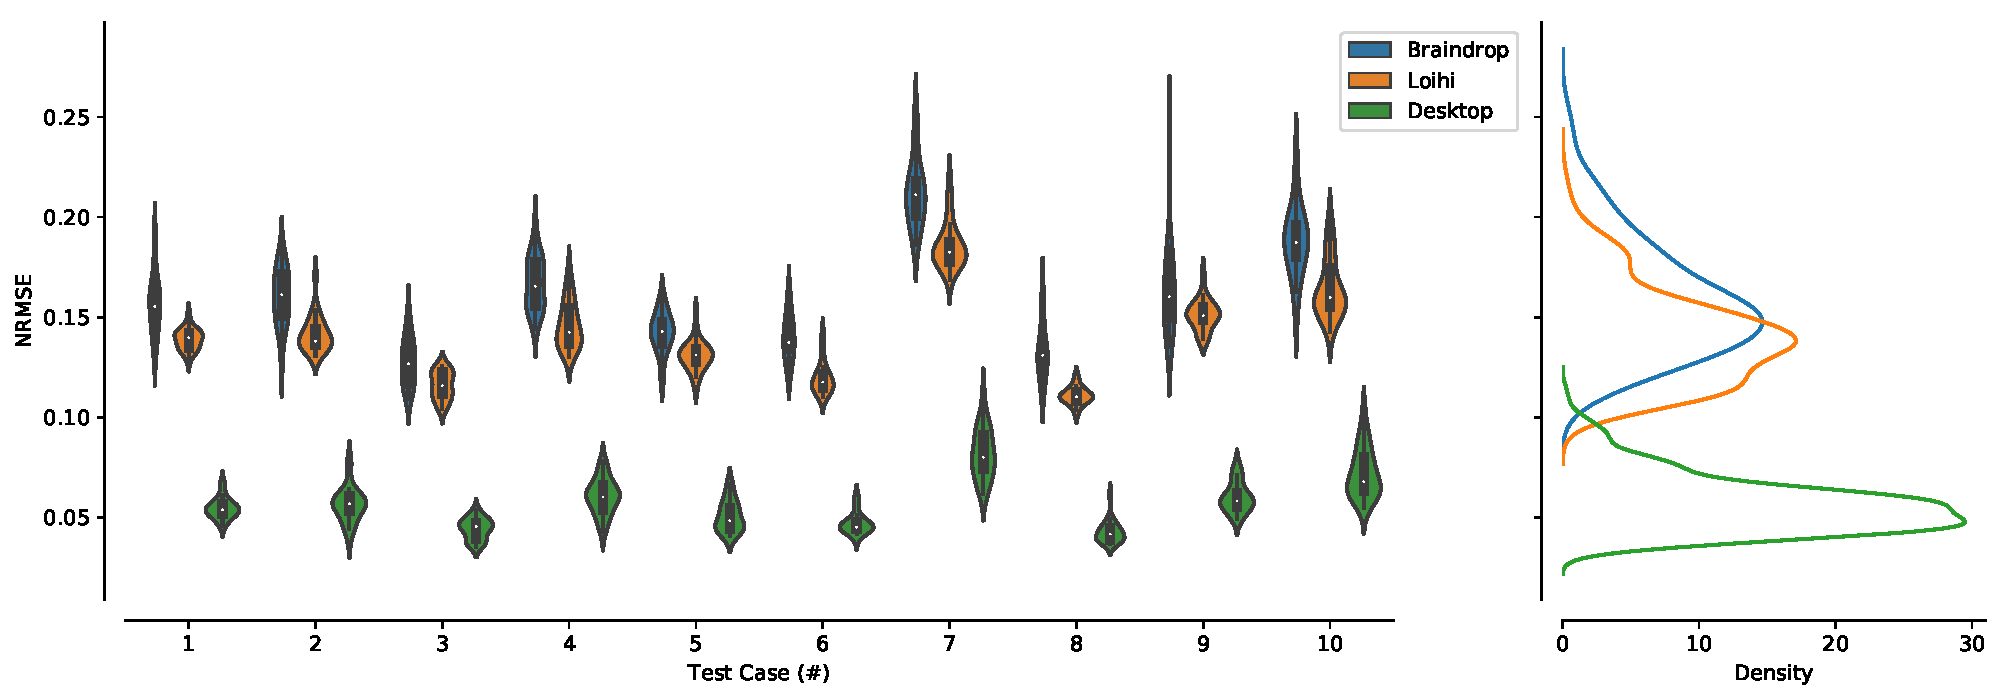
\includegraphics[width=\linewidth]{dn-trials}
    \caption{Overall Error}
    \label{fig:dn-trials}
  \end{subfigure}
  \caption[Dynamical memory on Braindrop and Loihi.]{ \label{fig:dn-neuromorphic}
    Delay Network~(DN; $q=3$, $\theta=100$\,ms; chapter~\ref{chapt:delays}) running on state-of-the-art neuromorphic hardware.
    (a)~Nengo Braindrop implementation, reproduced from \citet[][Figure~16]{braindrop2019}. 
    (b)~Nengo Loihi (v0.5.0) implementation.
    (c)~Overall error~(NRMSE) for Braindrop, Loihi, and a standard desktop CPU.
    The simulations of (a) and (b) correspond to a randomly chosen trial from the first test case from (c).
    Loihi simulations performed by Xuan Choo from Applied Brain Research, Inc.
    See text for details.
  }
\end{figure}

We now instantiate the same Delay Network~(DN) from chapter~\ref{chapt:delays} on state-of-the-art neuromorphic hardware (see Figure~\ref{fig:dn-neuromorphic}).
This system is an entirely different kind of dynamical system that persists not the input's sum, but finite windows of the input's history.
Specifically, the DN \emph{buffers} a sliding window of the input, thus serving as a continuous-time memory, and enabling the computation of arbitrary nonlinear transformations across a window of time.
This can be used as a basic building block for working memory models that must represent not only \emph{what} has occurred, but also \emph{when} it has occurred.

This system is described by (repeating equations~\ref{eq:delay-system}--\ref{eq:basis-functions}, for clarity):
\begin{equation*}
\begin{aligned}
  \theta \dot{\V{x}}(t) &= A\V{x}(t) + Bu(t) \\
  A &= \begin{pmatrix} -v_0 & -v_0 & \cdots & -v_0 \\ v_1 & 0 & \cdots & 0 \\ 0 & \ddots & \ddots & \vdots \\ 0 & 0 & v_{d-1} & 0\end{pmatrix} \\
  B &= \transpose{\begin{pmatrix} v_0 & 0 & \cdots & 0\end{pmatrix}} \\
 v_i &= (q+i)(q-i)(i+1)^{-1} \\ %and $w_i := (-1)^{d - 1 - i} \left( \frac{i+1}{d} \right)$
  u(t - \theta') &\approx \sum_{i=0}^{q-1} \mathcal{P}_{i,q} \left(\frac{\theta'}{\theta} \right) \, x_{q-1-i}(t) \text{,} \quad 0 \le \theta' \le \theta \\
\mathcal{P}_{i,q}(r) &= \begin{pmatrix}q \\ i\end{pmatrix}^{-1} \sum_{j=0}^i \begin{pmatrix}q \\ j\end{pmatrix} \begin{pmatrix}2q - 1 - j \\ i - j\end{pmatrix} \left( -r \right)^{i - j} \text{.} %\text{,}\quad 0 \le r \le 1 \text{,}\quad i = 0 \ldots d - 1
\end{aligned}
\end{equation*}
In addition, the state-space realization is balanced and normalized (see section~\ref{sec:software}), and the polynomial basis functions are rotated accordingly.

\TODO{Grab and plot the distribution from the calibration data using the mapped xy coordinates for the 3 ensembles.}

To implement the DN, three pools, each containing $128$ spiking LIF neurons, are recurrently coupled to each other (and to themselves), and trained to optimally buffer a white noise test signal---band-limited to $3$\,Hz---across a $100$\,ms sliding time-window.
Output spikes are filtered using a lowpass synapse with $\tau = 20$\,ms, and weighted to decode both the state-vector and the window of history via $\mathcal{P}_{i, 3}(\cdot)$. % using equation~\ref{eq:delay-readouts}.

For this experiment, we use identical Nengo model code for both neuromorphic backends.
On Braindrop~(see Figure~\ref{fig:dn-neuromorphic}~(a), reproduced from \citet[][Figure~16]{braindrop2019}),
the chip is configured to use the default distribution of synaptic time-constants (mean $\tau \approx 18$\,ms).
For Loihi~(see Figure~\ref{fig:dn-neuromorphic}~(b)), the recurrent time-constant is set to $\tau=10$\,ms, and weight matrices are unfactored.
We also compare this to the reference Nengo simulator ($\tau=10$\,ms) running the exact same model on a conventional desktop CPU, to obtain a baseline level of performance.
The overall error is evaluated across the entire delay interval $\theta' \in [0, \theta]$ using the corresponding analytical readout, $\mathcal{P}_{i, 3}(\cdot)$.

Table~\ref{tab:dn-neuromorphic} reports the bootstrapped 95\% confidence intervals across $25$ trials of $10$ separate test cases.
Given the inherent variability in Braindrop's analog computation, and its incredibly low power-consumption relative to both Loihi and the CPU solutions, it is surprisingly accurate given our anecdotal experience simulating noisy small-scale dynamical spiking networks.
However, these results reveal an unexpected drop in precision on Loihi relative to the reference CPU solution.
We attribute this to a combination of: the input's encoding into spikes, the LIF neuron model's discretization in time, quantization errors in neural states and recurrent weights, and the uniform ISIP criteria being systematically violated leading to state discrepancy (definition~\ref{def:state-discrepancy}).
Notably, this problem is revealed by fewer neurons per dimension, faster input frequencies, a faster system-level time-constant ($\theta$), and faster synaptic time-constant ($\tau$), relative to the previous experiment in section~\ref{sec:integrator}.
It is difficult to explore these issues without direct access to the hardware.
Future work is needed to ensure that high-bandwidth signals are being adequately and scalably encoded as per our analysis in chapter~\ref{chapt:analysis}.
%But all things considered, the accuracy of all of these methods is remarkable given that spiking reservoirs and FORCE networks cannot achieve these levels of accuracy for the same number of neurons, on a CPU, with additional memory, slower processing, and longer training times (see sections~\ref{sec:delay-rc} and~\ref{sec:force-comparison}).

\begin{table}
\centering
  \begin{tabular}{@{}lr@{}} \toprule
    Method & 95\% Confidence Interval \\
    \midrule
Braindrop & [0.156,~0.163] \\
Loihi & [0.146,~0.153] \\
Nengo-Loihi Emulator & [0.145, 0.151] \\
Reference CPU & [0.055,~0.059] \\
    \bottomrule
  \end{tabular}
  \caption[Delay Network benchmark on neuromorphic hardware.]{ \label{tab:dn-neuromorphic}
      Performance of the Delay Network~(DN) running on state-of-the-art neuromorphic hardware:
      Braindrop and Loihi.
      We also include Nengo's emulation of the Loihi hardware, and Nengo's CPU reference backend.
      All four simulations use the same model code and test signals.
  }
\end{table}
